\section{Database Architecture}

\subsection{Database Model}


This section illustrates the architecture of the database using a NoSQL database.
Figure 4.3 is a database ER Model which describes the tables created in the database.
We used MongoDB is a cross-platform document-oriented database program.
\newline
\begin{figure}[htp]%
    \center%
    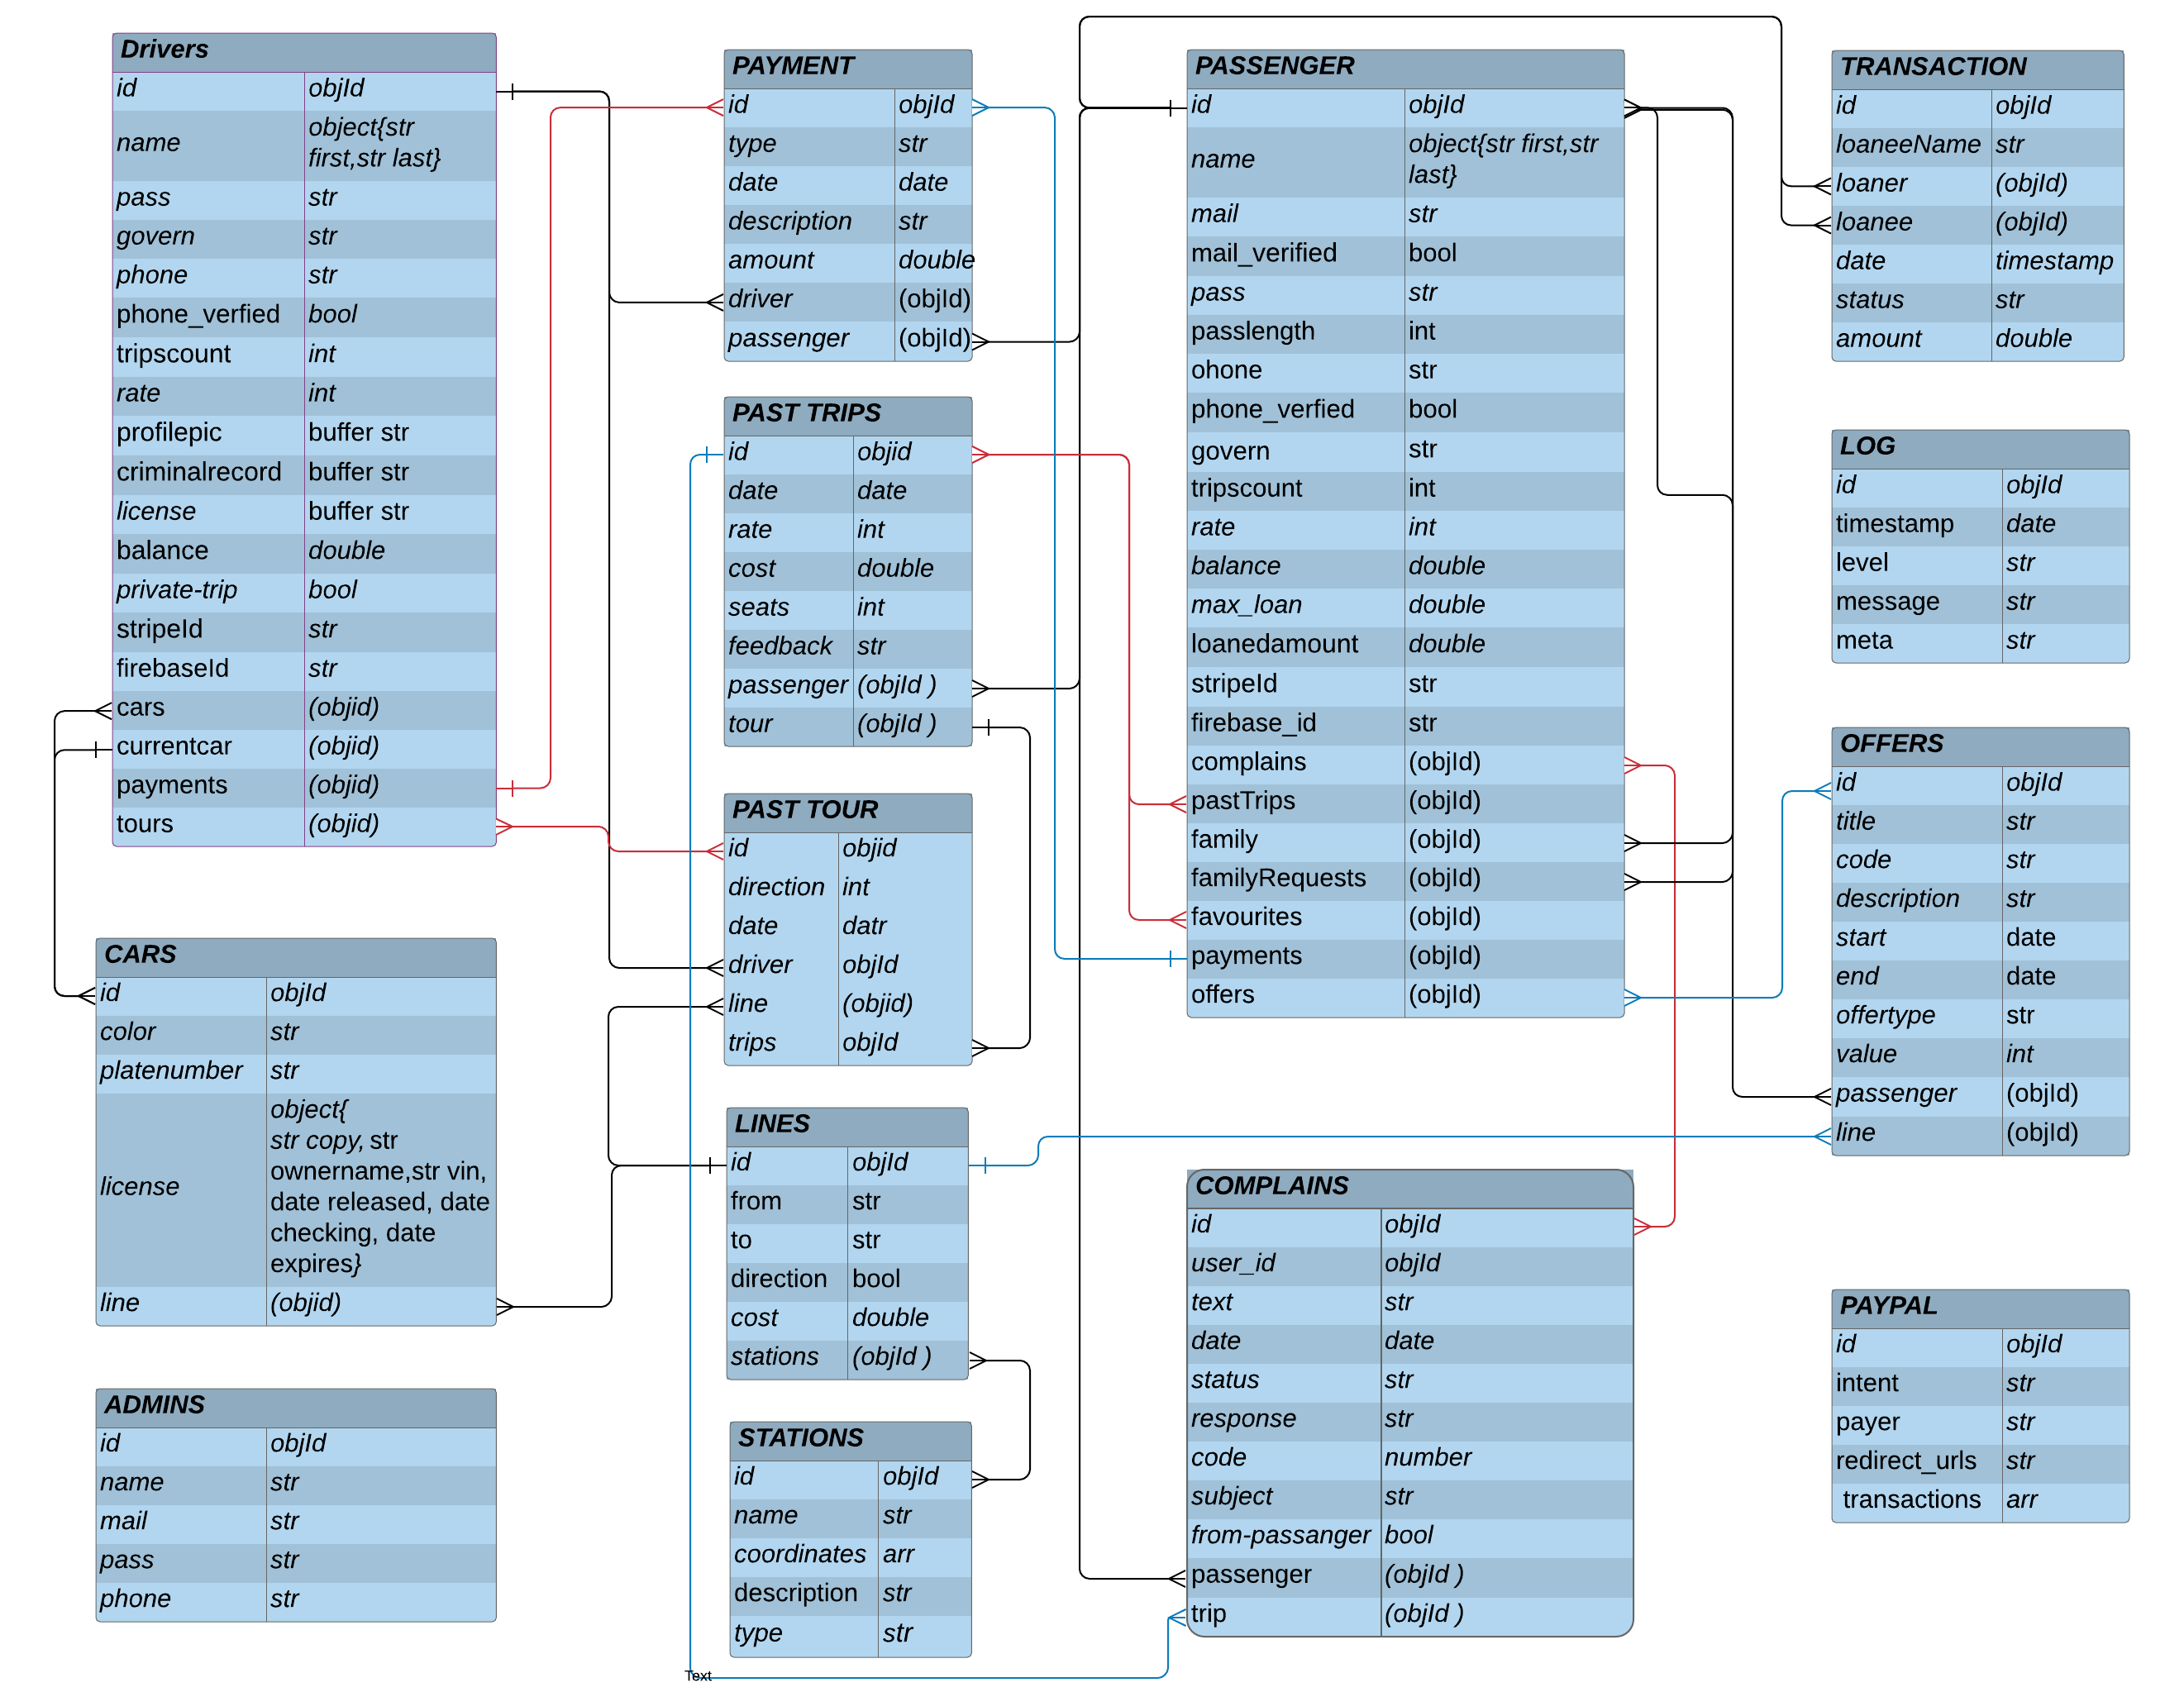
\includegraphics[width=1.1\textwidth]{images/ch4/db_model.png}%
     % you need to add the caption for the list of figures
    \caption[Database ER Model]{Database ER Model}\label{fig: Database ER Model}%
  \end{figure}
\newline

\newpage

\subsection{MongoDB}
\hspace{2cm}In this section, we will show why we use MongoDB Database?
 When We need to Database to store data in our application, we have two options to choose "SQL Database", "NoSQL Database (MongoDB)".

\textbf{The main differences between MongoDB and MySQL:}\\
MySQL is a relational database management system (RDBMS) from the Oracle Corporation. Like other relational systems, MySQL stores data in tables and uses structured query language (SQL) for database access. When MySQL developers need to access data in an application, they merge data from multiple tables together in a process called a join. In MySQL, you predefine your database schema and set up rules to govern the relationships between fields in your tables.\\

MongoDB is a NoSQL database that stores data as JSON-like documents. Documents store related information together and use the MongoDB query language (MQL) for access. Fields can vary from document to document - there is no need to declare the structure of documents to the system, as documents are self-describing. Optionally, schema validation can be used to enforce data governance controls over each collection.\\
\\
 \textbf{This is a comparison between them:} \cite{AF2}\\

 \begin{longtable}{||p{8cm}||p{8cm}||}
 \hline
 \textbf{SQL Database} & \textbf{NoSQL Database (MongoDB)} \\  
 \hline\hline
 Relational database & Non-relational database  \\ 
 \hline
 Supports SQL query language & Supports JSON query language \\
 \hline
 Table based & Collection based and key-value pair \\
 \hline
 Row based & Document based  \\
 \hline
 Column based & Field based \\ 
 \hline
 Support foreign key & No support for foreign key\\ 
 \hline 
 Support for triggers & No Support for triggers\\
 \hline
 Contains schema which is predefined & Contains dynamic schema\\
 \hline
 Not fit for hierarchical data storage & Best fit for hierarchical data storage\\
 \hline
 Vertically scalable - increasing RAM & Horizontally scalable - add more servers\\
 \hline
 Emphasizes on ACID properties (Atomicity, Consistency, Isolation and Durability) & Emphasizes on CAP theorem (Consistency, Availability and Partition tolerance)\\
 \hline
 \caption{Comparison between SQL and NoSQL database}
\end{longtable}\\

Organizations of all sizes are adopting MongoDB, especially as a cloud database, because it enables them to build applications faster, handle highly diverse data types, and manage applications more efficiently at scale.\\
Thousands of companies like Bosch, Barclays, and Morgan Stanley run their businesses on MongoDB, and use it to handle their most demanding apps in areas like IoT, Gaming, Logistics, Banking, e-Commerce, and Content Management.\\

Development is simplified as MongoDB documents map naturally to modern, object-oriented programming languages. Using MongoDB removes the complex object-relational mapping (ORM) layer that translates objects in code to relational tables. MongoDB’s flexible data model also means that your database schema can evolve with business requirements. MySQL's rigid relational structure adds overhead to applications and slows developers down as they must adapt objects in code to a relational structure.\\

MongoDB can also be scaled within and across multiple distributed data centers, providing new levels of availability and scalability previously unachievable with relational databases like MySQL. As your deployments grow in terms of data volume and throughput, MongoDB scales easily with no downtime, and without changing your application. In contrast, achieving scale with MySQL often requires significant custom engineering work.\\

\textbf{MongoDB is a great choice if you need to:}\\
Represent data with natural clusters and variability over time or in its structure
Support rapid iterative development.
Enable collaboration of a large number of teams
Scale to high levels of read and write traffic.
Scale your data repository to a massive size.
Evolve the type of deployment as the business changes.
Store, manage, and search data with text, geospatial, or time series dimensions.\cite{AF3}

\subsection{Firebase Realtime Database}

\hspace{2cm}We faced a problem with our need to continuously update data as we needed process data in real-time.\\
As the data of drivers and trips in our application need to be updated in real-time like available drives, the number of seats, and locations of drivers.

So we use firebase real-time database to solve this problem.

Firebase is a mobile and web application development platform developed by Firebase, Inc. in 2011, then acquired by Google in 2014.\cite{AF5}

\newline
\begin{figure}[htp]%
    \center%
    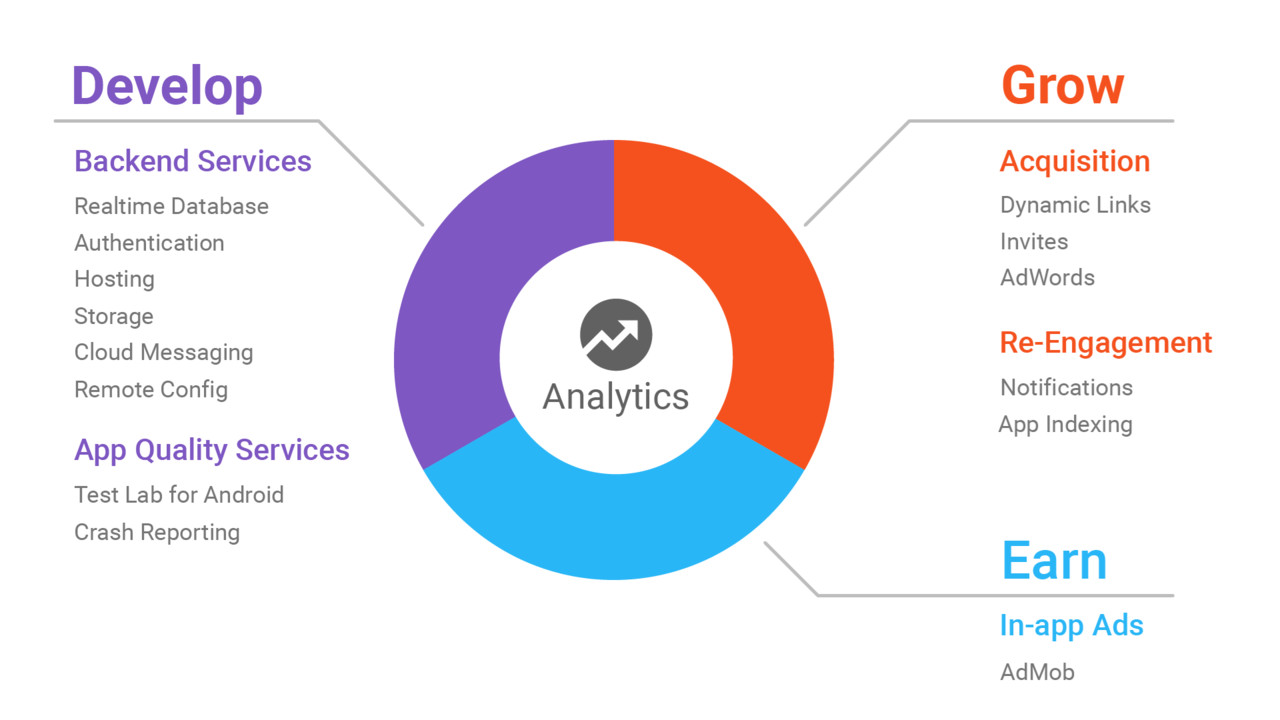
\includegraphics[width=1\textwidth]{images/ch4/firebase.png}%
     % you need to add the caption for the list of figures
    \caption[Firebase Features]{Firebase Features}\label{fig: Firebase Features}%
  \end{figure}
\newline




The main goal of the system is to provide a secure, reliable and fast way to synchronize data with a minimal amount of coding effort on the part of the developer. The database system is also designed to scale to support millions of users.

The database is referred to as being “realtime” because the speed with which the data is synchronized across clients is probably as close to realtime as is currently achievable (taking into consideration the physical limitation of transmitting data over the internet and wireless connections). The elapsed time while a data change on one client propagates to another is visually imperceptible.

The Realtime Database also provides data persistence by storing data locally, thereby enabling the data to remain accessible even when a device is offline. When connectivity is re-established, the local data is automatically synchronized and merged with the remote data.\cite{AF4}

\newline
\begin{figure}[htp]%
    \center%
    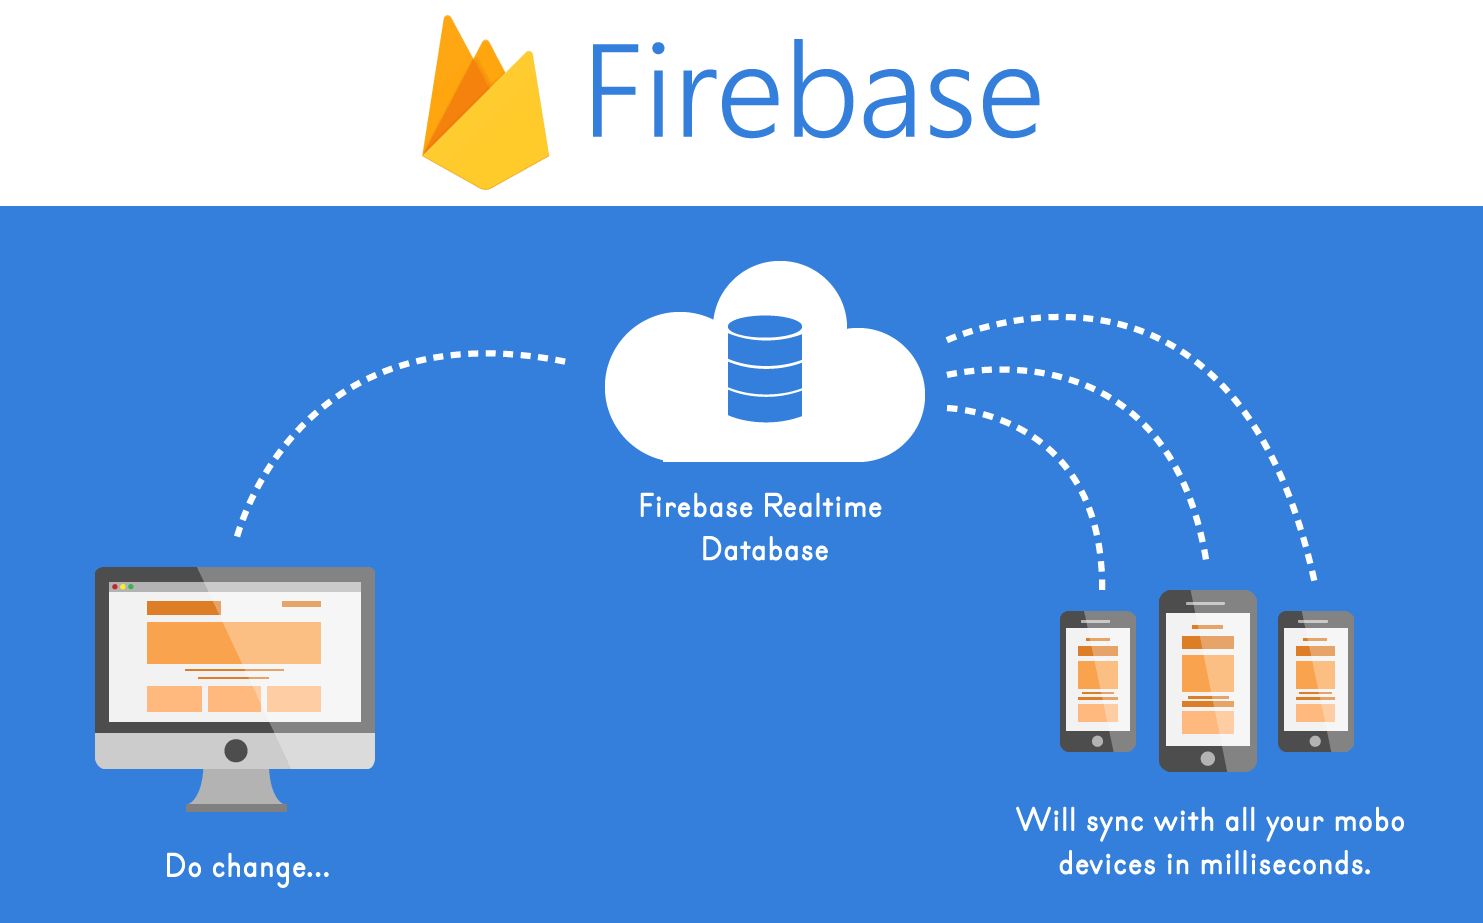
\includegraphics[width=0.8\textwidth]{images/ch4/firebasecon.png}%
     % you need to add the caption for the list of figures
    \caption[Firebase Process]{Firebase Process}\label{fig: Firebase  Process}%
  \end{figure}
\newline
















